\section{Resultados}
\label{sec:res}

\subsection{Parámetros identificados}
La Tabla~\ref{tab:par} reúne los parámetros y la Fig.~\ref{fig:ident} los datos de los ensayos. Las inercias cumplen $I_x<I_y<I_z$ con incertidumbres estándar combinadas de $1.4$, $1.6$ y $2.2$\,\% (Anexo~A); $I_z$ es la más dispersa porque sus cinco períodos van de 4.28 a 4.54\,s. Además $I_x+I_y$ difiere de $I_z$ en un $0.9$\,\%, compatible con cero, como se espera de un cuerpo casi plano. Con ellas, la autoridad de roll en hover es de $0.34$\,N\,m, equivalente a unos $35$\,rad/s$^2$ ($\approx2000^\circ$/s$^2$), calculada con los parámetros del firmware. Con $\omega_{\max}=1046$\,rad/s el empuje máximo es $14.05$\,N (relación empuje/peso $1.43$) y el hover cae en el $70$\,\% del acelerador. Con $k_fl/k_m=10.2$, el yaw es diez veces más caro que el roll en rango de motor.

\begin{table}[t]
\caption{Parámetros del dron. Incertidumbre estándar combinada (Anexo~A).}
\label{tab:par}
\centering\footnotesize\setlength{\tabcolsep}{3pt}
\begin{tabular}{@{}lll@{}}
\toprule
Parámetro & Valor & Unidad \\
\midrule
Masa $m$ & 1.0022 & kg \\
Brazo efectivo $l$ & 0.1616 & m \\
$I_x$ & $(9.71\pm0.13)\times10^{-3}$ & kg\,m$^2$ \\
$I_y$ & $(10.56\pm0.17)\times10^{-3}$ & kg\,m$^2$ \\
$I_z$ & $(20.08\pm0.45)\times10^{-3}$ & kg\,m$^2$ \\
$K_f$ (hoja, 1000--1500\,\textmu{}s) & $3.91\times10^{-6}$ & N/\textmu{}s$^2$ \\
$a$ (ajuste cuadrático, 13 pts) & $(3.42\pm0.34)\times10^{-6}$ & N/\textmu{}s$^2$ \\
$K_m=\alpha^2K_f$ (hoja) & $6.19\times10^{-8}$ & N\,m/\textmu{}s$^2$ \\
$K_m=\alpha^2a$ (ajuste, Anexo~A) & $(5.42\pm0.53)\times10^{-8}$ & N\,m/\textmu{}s$^2$ \\
$k_f$ (firmware) & $3.2107\times10^{-6}$ & N/(rad/s)$^2$ \\
$k_m$ (firmware) & $5.088\times10^{-8}$ & N\,m/(rad/s)$^2$ \\
\bottomrule
\end{tabular}
\end{table}

\begin{figure*}[t]
\centering
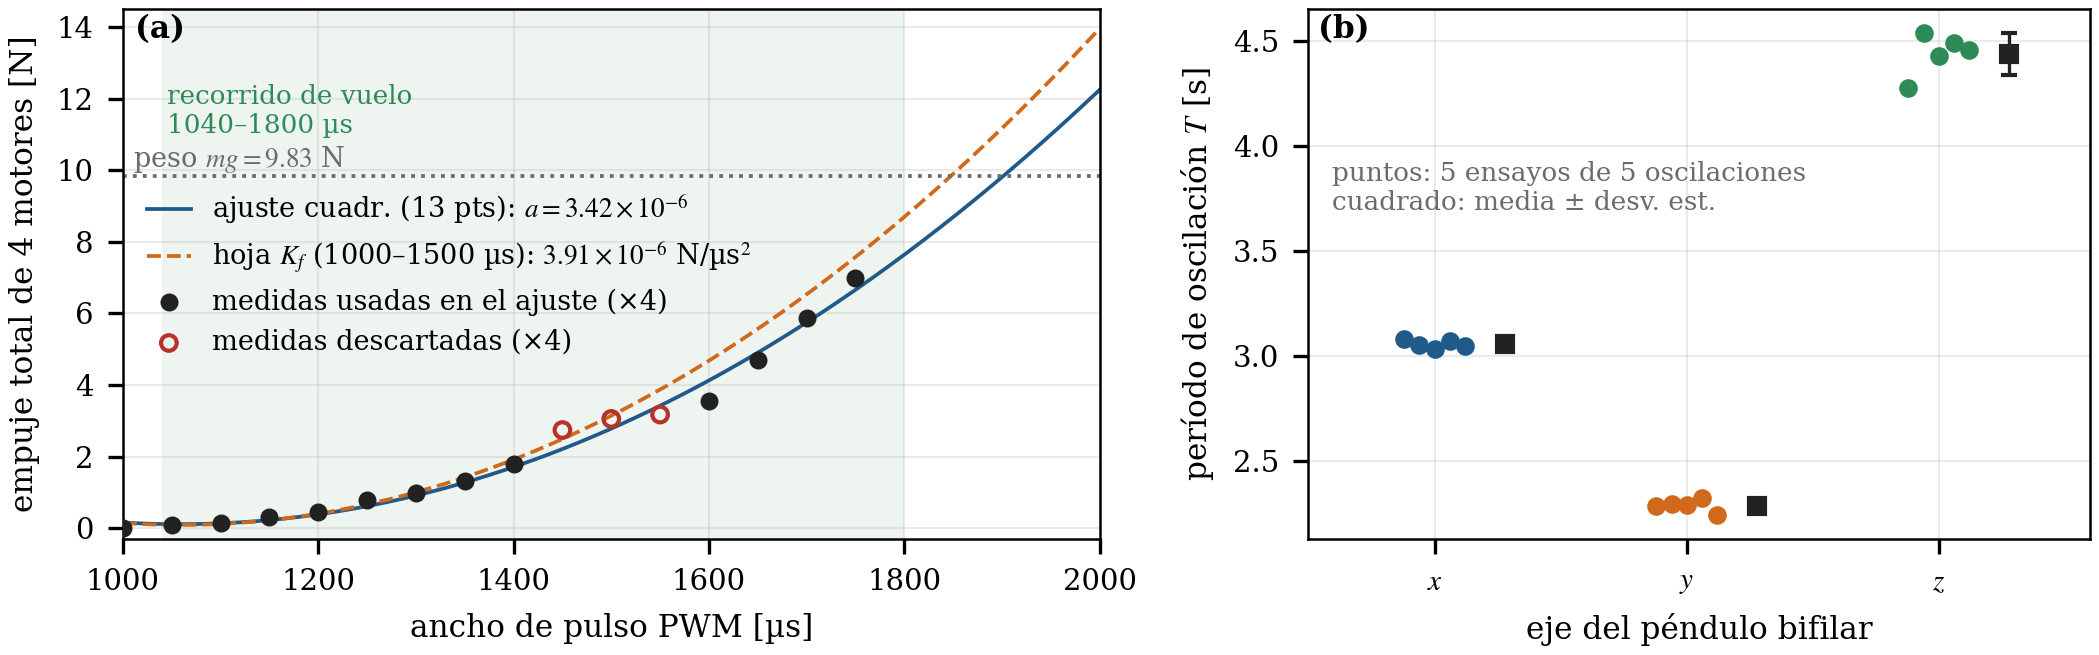
\includegraphics[width=0.93\textwidth]{f_ident.png}
\caption{Ensayos de identificación. (a) Empuje total (cuatro motores) frente al pulso PWM, con el ajuste cuadrático y la curva de la hoja. (b) Períodos medidos en el péndulo bifilar.}
\label{fig:ident}
\end{figure*}

El coeficiente $K_f$ depende del rango de ajuste: la hoja da $3.91\times10^{-6}$ usando los puntos de 1000 a 1500\,\textmu{}s y el ajuste cuadrático de los 13 puntos filtrados da $3.42\times10^{-6}$, un $12.5$\,\% menos ($R^2=0.987$ y $0.992$). La diferencia crece al extrapolar: a 2000\,\textmu{}s predicen $13.8$ y $12.2$\,N en total. Más importante, la curva de banco no es transferible al vuelo. En el vuelo B los cuatro motores trabajaron en promedio al $87$\,\% del recorrido, unos $1700$\,\textmu{}s, donde la curva de banco da $5.7$--$6.4$\,N en total, menos que el peso ($9.83$\,N), y sin embargo el dron voló. Las causas posibles son la recalibración de los ESC a 1040--1800\,\textmu{}s, la tensión de batería durante el ensayo y la medición con balanza; los datos no permiten separarlas. El firmware evita el problema suponiendo $\omega$ lineal en el recorrido calibrado y tratando $\omega_{\max}$ como parámetro de ajuste.

\subsection{Vuelos con V\_11: actitud}
La Fig.~\ref{fig:vueloB} muestra el vuelo B y la Tabla~\ref{tab:vuelos} resume los dos vuelos. En B el empuje se aplicó en $t=0.9$\,s, el dron superó 0.3\,m en $3.3$\,s y alcanzó $1.48$\,m en $5.6$\,s. Después descendió lentamente desde $\approx0.6$\,m ($t\approx8$\,s) hasta tocar el suelo en $t\approx19.4$\,s.

\begin{figure}[t]
\centering
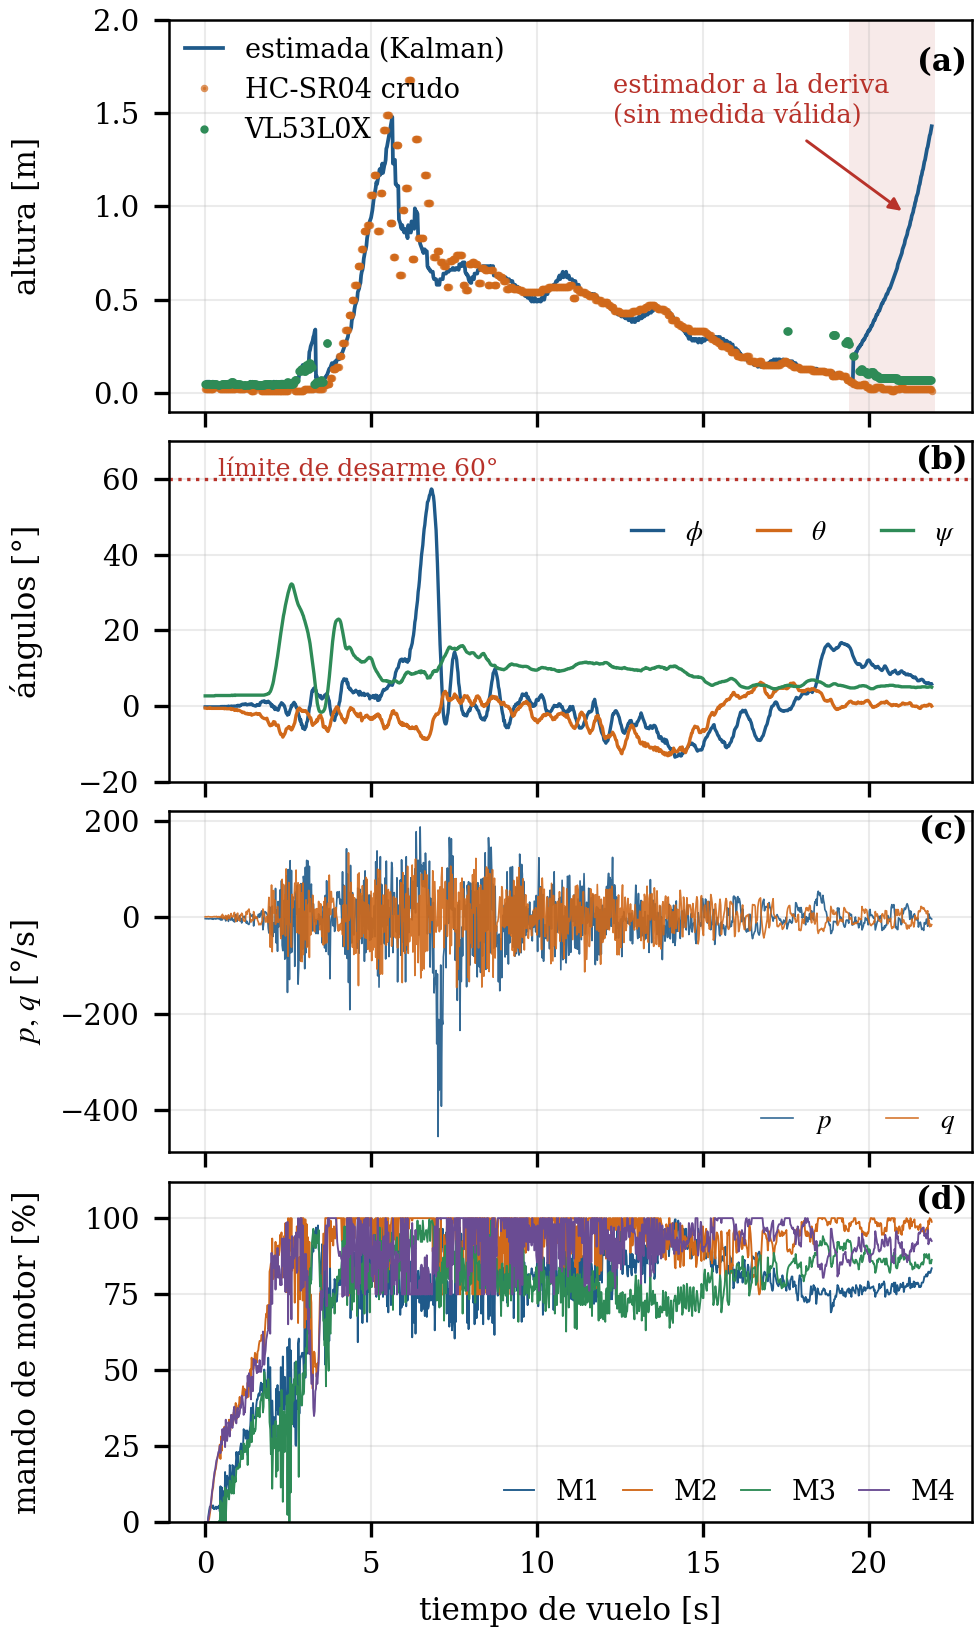
\includegraphics[width=0.97\linewidth]{f_vuelo_B.png}
\caption{Vuelo B (V\_11): (a) altura estimada y sensores; (b) ángulos de Euler; (c) velocidades angulares $p$ y $q$; (d) mando de cada motor. La banda roja marca el tramo sin medida válida tras la toma de contacto.}
\label{fig:vueloB}
\end{figure}

\begin{table}[t]
\caption{Métricas de los vuelos V\_11 (muestras con altura $>0.15$\,m).}
\label{tab:vuelos}
\centering\footnotesize\setlength{\tabcolsep}{3pt}
\begin{tabular}{@{}lcc@{}}
\toprule
Métrica & A & B \\
\midrule
Duración registrada [s] & 21.0 & 33.0 \\
Muestras en el aire & 578 & 808 \\
Altura estimada máxima [m] & 1.77 & 1.48 \\
Roll: media / desv. / máx. [$^\circ$] & 8.9 / 5.4 / 18.9 & 2.2 / 11.5 / 57.4 \\
Pitch: media / desv. / máx. [$^\circ$] & $-7.5$ / 3.1 / 15.8 & $-2.6$ / 4.5 / 13.1 \\
Tiempo con $|\phi|<10^\circ$ [\%] & 51 & 78 \\
$\sigma_p,\sigma_q,\sigma_r$ [$^\circ$/s] & 49 / 45 / 14 & 62 / 44 / 14 \\
Mezclador saturado [\%] & 11 & 16 \\
Motor 2 / motor 4 al $\ge99$\,\% [\%] & 43 / 0 & 37 / 25 \\
Empuje pedido medio [N] & 9.59 & 11.33 \\
\bottomrule
\end{tabular}
\end{table}

La actitud se mantuvo acotada en ambos vuelos, sin desarmes por inclinación. En B, el $90$\,\% del tiempo estuvo con $|\theta|<10^\circ$ y el $78$\,\% con $|\phi|<10^\circ$. Hay un evento relevante: un pico de roll de $57.4^\circ$ en $t=6.8$\,s (con $|p|$ hasta unos $450^\circ$/s), a $2.6^\circ$ del umbral de desarme de $60^\circ$, que se recuperó en menos de un segundo (el roll estuvo $0.62$\,s por encima de $30^\circ$). El yaw se mantuvo entre $-1.6^\circ$ y $32^\circ$ y presenta dos excursiones al despegar, de $32^\circ$ y $23^\circ$. En A el roll y el pitch tienen medias de $+8.9^\circ$ y $-7.5^\circ$; como el CSV no guarda la referencia de actitud, no se puede separar si es error de seguimiento, un nivel (trim) mal ajustado o una orden del piloto.

El contenido espectral (vuelo B, $t=4.5$--$21.9$\,s) muestra que la oscilación no es de baja frecuencia: el $82$--$90$\,\% de la varianza de $\phi$ y $\theta$ está bajo 1\,Hz, pero el $82$\,\% de la de $q$ está entre 8 y 25\,Hz. Las desviaciones de 44--62$^\circ$/s en $p$ y $q$ (Fig.~\ref{fig:vueloB}c) serían entonces sobre todo ruido y vibración del giroscopio realimentados al mezclador, lo que se refleja en un mando de motor muy movido (Fig.~\ref{fig:vueloB}d). Es una interpretación: la caja negra muestrea a 50\,Hz, de modo que el contenido por encima de 25\,Hz se pliega sobre la banda observada, y no hay un registro a 250\,Hz con el que confirmarlo.

\subsection{Actuación y saturación}
El mezclador estuvo saturado el 11\,\% (A) y el 16\,\% (B) de las muestras en el aire, y el motor 2 trabajó al $\ge99$\,\% del recorrido el 43 y el 37\,\% del tiempo (el motor 4 el 25\,\% en B). La prioridad de V\_9 protege roll y pitch frente al yaw, pero no crea margen: el hover exige $\approx70$\,\% del acelerador y el empuje pedido medio fue de 9.6 y 11.3\,N ($68$ y $80$\,\%), de modo que en B queda poca reserva para corregir. En la fase de descenso lento de B ($t=8$--$19.4$\,s, altura $0.59\to0.06$\,m, $\bar{\dot z}=-0.05$\,m/s) el empuje pedido fue constante a $11.4$\,N, un $16$\,\% sobre $mg$; en el vuelo A, en un tramo de descenso lento ($t=13$--$16.7$\,s, altura $0.79\to0.45$\,m, $\bar{\dot z}=-0.03$\,m/s) fue de $7.8$\,N, un $21$\,\% bajo $mg$. El empuje de hover \emph{pedido} cambió un $46$\,\% entre dos vuelos del mismo día. Como el dron no mide la tensión de batería, el registro no permite atribuirlo a su descarga.

\subsection{Altura: lazo cerrado y estimador}
La Fig.~\ref{fig:holdA} muestra el único tramo en MANTENER ALTURA de los dos vuelos V\_11 (A, $t=0.78$--$3.38$\,s, 120 muestras). El modo se activó con el dron subiendo a $\approx0.65$\,m/s y $11.0$\,N, de modo que la ec. (\ref{eq:altura}) aprendió $g_{ef}\approx11$\,m/s$^2$ ($\approx1.1\,g$) como si fuera el hover. La altura estimada superó la referencia (0.36\,m y luego 0.96\,m) hasta 1.16\,m, y el error cuadrático medio en el tramo es de $0.24$\,m (máximo $0.60$\,m). Con un solo tramo de 2.6\,s no se puede afirmar que el lazo de altura cumpla su diseño ($\omega_n=2$\,rad/s). La prealimentación aprendida solo es válida si el modo se activa cerca del hover.

\begin{figure}[t]
\centering
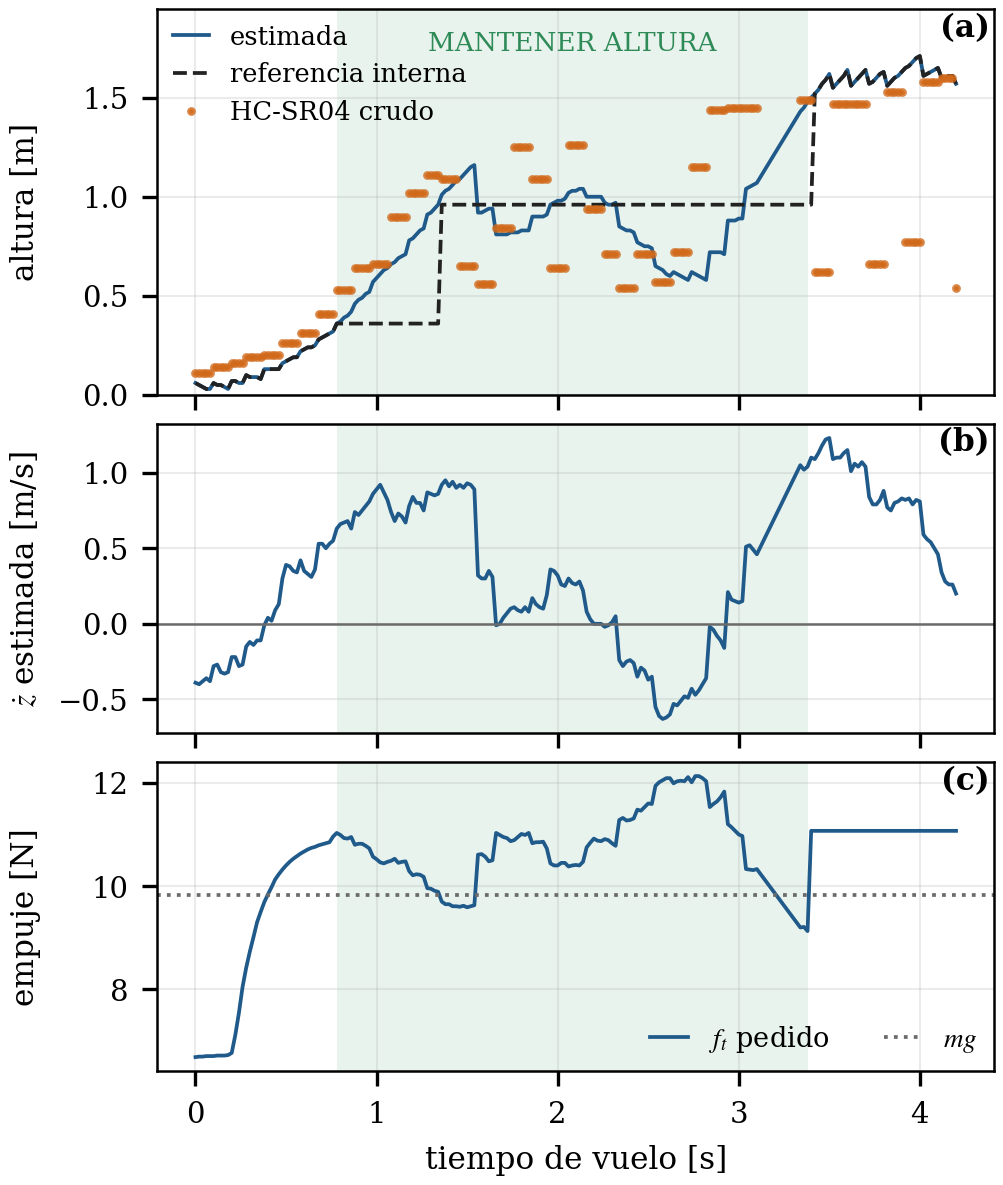
\includegraphics[width=0.93\linewidth]{f_hold_A.png}
\caption{Vuelo A (V\_11), modo MANTENER ALTURA (banda verde): (a) altura, (b) velocidad vertical estimada, (c) empuje pedido.}
\label{fig:holdA}
\end{figure}

La Tabla~\ref{tab:est} compara el estimador de altura entre versiones usando como indicador la diferencia con la lectura del ultrasonido y la fracción de muestras con altura estimada negativa, físicamente imposible. En el vuelo V\_10 de las 16:50 la altura estimada oscila con amplitud de varios metros alrededor de lecturas de ultrasonido de $0.3$--$1$\,m (Fig.~\ref{fig:estimador}a) y el $35$\,\% de las muestras tiene altura negativa; los otros cuatro vuelos de V\_10/V\_10b son mejores ($0.26$--$0.58$\,m). En V\_11-B la desviación es de $0.12$\,m y solo el $1$\,\% de las muestras difiere más de $0.5$\,m. Por encima de $0.8$\,m el ultrasonido crudo se aparta mucho de la altura estimada ($\approx0.3$--$0.4$\,m, frente a los $0.13$--$0.18$\,m del modelo $\sigma_{US}$); la puerta de innovación hace el resto.

\begin{table}[t]
\caption{Estimador de altura frente a la lectura del ultrasonido.}
\label{tab:est}
\centering\small
\begin{tabular}{@{}lccc@{}}
\toprule
Vuelo & Desv. [m] & $|\mathrm{res}|>0.5$\,m [\%] & Alt.\,$<0$ [\%] \\
\midrule
V\_10, 16:50 & 1.39 & 36.8 & 34.7 \\
V\_10, 17:42 & 0.31 & 7.6 & 2.3 \\
V\_10, 17:45 & 0.26 & 3.2 & 0.0 \\
V\_10b, 18:32 & 0.39 & 4.5 & 0.6 \\
V\_10b, 18:36 & 0.58 & 23.6 & 2.1 \\
V\_11, A (19:09) & 0.30 & 11.8 & 8.3 \\
V\_11, B (19:25) & 0.12 & 1.0 & 0.0 \\
\bottomrule
\end{tabular}
\end{table}

\begin{figure}[t]
\centering
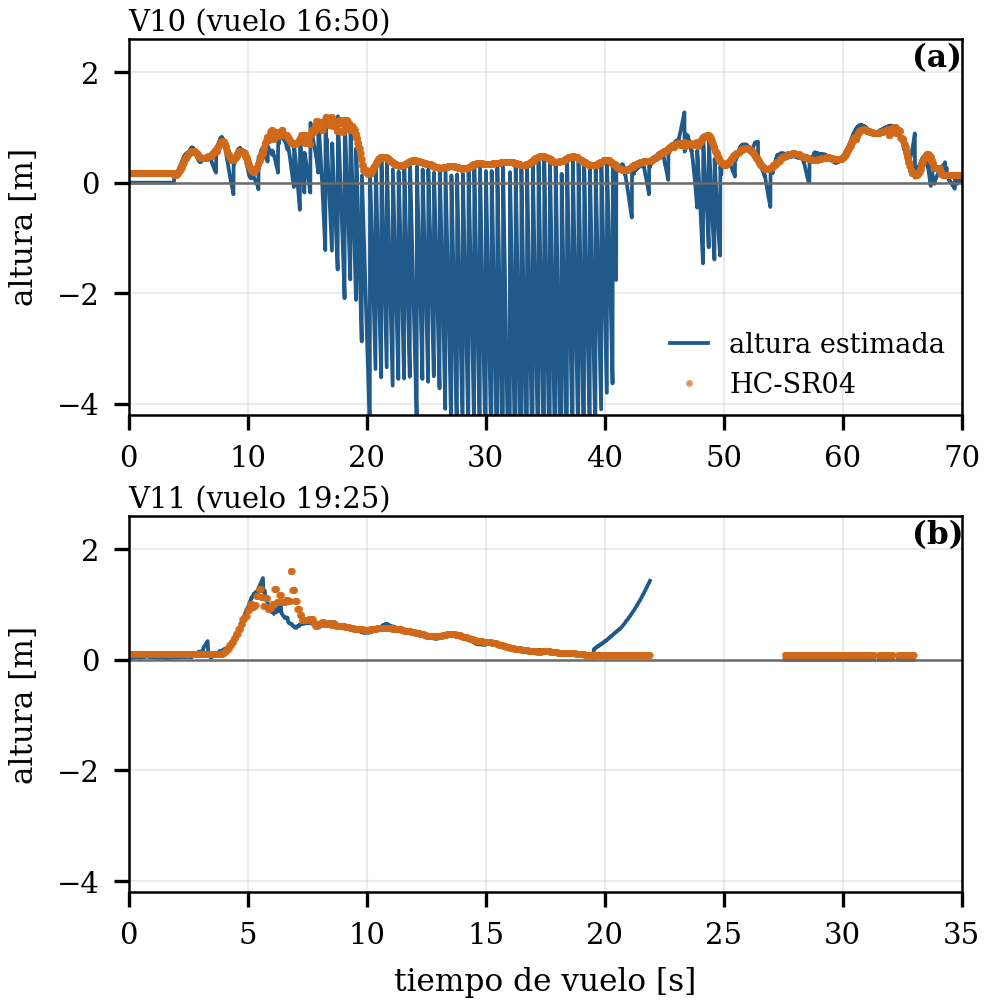
\includegraphics[width=0.93\linewidth]{f_estimador.png}
\caption{Altura estimada y lectura del ultrasonido: (a) V\_10, con oscilaciones del estimador por debajo del suelo; (b) V\_11 (vuelo B).}
\label{fig:estimador}
\end{figure}

La mejora no es uniforme. En V\_11-A hay un $8$\,\% de muestras negativas y en ambos vuelos V\_11 el estimador falla al final. En B, tras tocar el suelo ($t=19.4$\,s) el ultrasonido crudo lee $0.02$--$0.05$\,m, bajo su mínimo válido de $0.08$\,m; el ToF registra $0.07$--$0.10$\,m, pero el log marca \texttt{alt\_ok}=0 desde $t=20.6$\,s. Con el empuje aún en $11.4$\,N, la estimación sube de $0.06$ a $1.34$\,m en 2.4\,s, como si integrara la aceleración sin ancla (Fig.~\ref{fig:vueloB}a). En A ocurre lo contrario: tras $t=19.6$\,s (\texttt{alt\_ok}=0, con el ToF leyendo $0.05$--$0.06$\,m) la altura estimada cae hasta $-1.0$\,m. Las columnas registradas no permiten explicar por qué el ToF no ancla el filtro. Con dos vuelos V\_11 la comparación con V\_10 es indicativa, no concluyente.

\subsection{Discusión y limitaciones}
\label{sec:disc}
\emph{Qué funcionó.} La cascada de actitud del curso, con los parámetros identificados, bastó para despegar, subir a $1.5$\,m y volver al suelo sin desarme por inclinación en vuelos de 20--30\,s. El mezclador por prioridad y el Kalman re-sintonizado atienden los dos problemas que mostraron los registros de V\_9 y V\_10, el segundo con mejora parcial.

\emph{Qué no está demostrado.} (i) El lazo de altura cerrado solo tiene 2.6\,s de datos y con un error rms de $0.24$\,m. (ii) Las extensiones del curso (super-twisting y adaptación RLS) están implementadas y se describen, pero el CSV no registra su estado ni $\hat g$ ni $w$, y por defecto están apagadas: no hay evidencia de vuelo de que mejoren el resultado. (iii) El estimador diverge cuando el log marca \texttt{alt\_ok}=0 junto al suelo.

\emph{Limitaciones del modelo y de la instrumentación.} Hay una brecha de $K_f$ y empuje entre banco y vuelo; el empuje de hover pedido varió un $46$\,\% entre vuelos; no hay medición de batería ni de posición lateral; sin magnetómetro el yaw deriva; y el PWM a 50\,Hz limita el ancho de banda del lazo interno. La consecuencia práctica es poca reserva de empuje: el motor 2 trabaja al $\ge99$\,\% del recorrido entre el 37 y el 43\,\% del tiempo.
